\documentclass[conference]{IEEEtran}
\IEEEoverridecommandlockouts

\usepackage{cite}
\usepackage{amsmath,amssymb,amsfonts}
\usepackage{algorithmic}
\usepackage{graphicx}
\usepackage{textcomp}
\usepackage{xcolor}
\usepackage{booktabs}
\usepackage{multirow}

\def\BibTeX{{\rm B\kern-.05em{\sc i\kern-.025em b}\kern-.08em
    T\kern-.1667em\lower.7ex\hbox{E}\kern-.125emX}}

\begin{document}

\title{Short-Window Synthetic Speech Detection under\\Telephone-Channel Degradation\\
{\footnotesize \textsuperscript{*}These authors contributed equally to this work.}}

\author{%
\IEEEauthorblockN{Krishnapriya Vinod Pillai\textsuperscript{*}}
\IEEEauthorblockA{\textit{Dept.\ of Mechanical Engineering}\\
\textit{Amrita Vishwa Vidyapeetham}\\
Bengaluru, India\\
bl.en.u4rae23019@bl.students.amrita.edu}
\and
\IEEEauthorblockN{Nihaarika H\textsuperscript{*}}
\IEEEauthorblockA{\textit{Dept.\ of Mechanical Engineering}\\
\textit{Amrita Vishwa Vidyapeetham}\\
Bengaluru, India\\
bl.en.u4rae23028@bl.students.amrita.edu}
\and
\IEEEauthorblockN{Podilapu Srinidhi\textsuperscript{*}}
\IEEEauthorblockA{\textit{Dept.\ of Mechanical Engineering}\\
\textit{Amrita Vishwa Vidyapeetham}\\
Bengaluru, India\\
bl.en.u4rae23031@bl.students.amrita.edu}
\and
\IEEEauthorblockN{Kumaran U}
\IEEEauthorblockA{\textit{Dept.\ of Computer Science}\\
\textit{Amrita Vishwa Vidyapeetham}\\
Bengaluru, India\\
kumaran@blr.amrita.edu}
}

\maketitle

% ============================================================
\begin{abstract}
The growing availability of speech-synthesis and voice-cloning technologies has introduced new risks in telephone-based social-engineering attacks. AI-generated speech can be used to impersonate trusted callers such as bank representatives and persuade victims to disclose sensitive financial information. This work studies short-window synthetic speech detection under telephone-channel degradation, with a limited external evaluation on vishing-style calls. A Mel-spectrogram convolutional neural network (Mel-CNN) is compared with MFCC-based Logistic Regression (LR), Random Forest (RF) and Support Vector Machine (SVM) baselines. All models are trained on the ASVspoof 2019 Logical Access corpus using a 1\,s window and evaluated with thresholds frozen on the development set. Under clean conditions the Mel-CNN achieves an equal error rate (EER) of 22.4\%, versus 33--36\% for the baselines. Under simulated telephone-channel conditions (300--3400\,Hz band-pass, 8\,kHz resampling, G.711 A-law) the clean-trained CNN degrades to 31.7\% EER. Channel-aware training (mixed clean, telephone and codec conditions) recovers to 27.9\% EER on telephone. A streaming evaluation with four temporal-aggregation rules shows that a 1\,s window is sufficient for the first spoof decision, with a median spoof-call alarm at 2\,s. External evaluation on a 40-call vishing-style subset (VISHGUARD) and on the DEEP-VOICE cloned-speech corpus yields near-chance results, indicating that in-domain ASVspoof features do not transfer to these conditions.
\end{abstract}

\begin{IEEEkeywords}
synthetic speech detection, voice cloning, vishing, telephone-channel robustness, short-window detection, ASVspoof, convolutional neural network
\end{IEEEkeywords}

% ============================================================
\section{Introduction}

Voice phishing (vishing) is a growing cybersecurity threat. An adversary impersonates a trusted party---a bank representative, government official, or family member---to manipulate a victim into disclosing credentials or authorizing a financial transfer. Modern text-to-speech and voice-cloning systems have made synthetic speech realistic enough that listeners frequently cannot distinguish it from genuine speech.

The banking domain is particularly exposed: telephone interactions routinely involve account verification, card activity, and identity confirmation. Existing fraud controls rely on transaction behavior or caller metadata and do not examine whether the voice is synthetic.

Spoofed-speech detection has been studied extensively on benchmarks such as ASVspoof. Practical telephone deployment adds two challenges. First, bandwidth limitation, resampling, and codec distortion cause distribution shift for detectors trained on clean speech. Second, a live system cannot wait for a full recording; it must update its risk estimate from short, incoming segments.

This work addresses three questions:
\begin{enumerate}
  \item How well can a 1\,s-window Mel-CNN separate bona fide and AI-generated speech under clean conditions compared with hand-crafted feature baselines?
  \item How does a clean-trained detector degrade under simulated telephone-channel conditions, and how much does channel-aware training recover?
  \item Can short-window processing with temporal aggregation support early detection on ASVspoof streams, and does the detector transfer to external vishing-style and voice-clone data?
\end{enumerate}

The main contributions are:
\begin{itemize}
  \item A short-window preprocessing pipeline respecting the official ASVspoof 2019 train/development/evaluation split, with thresholds frozen on the development set.
  \item Simulation of telephone degradation using band limitation, resampling and G.711 A-law processing, and an ablation across five training regimes and seven test conditions.
  \item A feature-set comparison of MFCC, spectral descriptors and F0 features with LR, RF and SVM classifiers.
  \item A streaming framework with 1\,s windows and 0.5\,s hop, using four aggregation rules with $\tau$ selected on the development set at a target FPR of 10\%.
  \item An external evaluation on a 40-call vishing-style subset (VISHGUARD) and on DEEP-VOICE cloned speech, reported as negative transfer results.
\end{itemize}

% ============================================================
\section{Related Work}

\textbf{Spoofing datasets.}
The ASVspoof 2019 Logical Access corpus~\cite{asvspoof2019} provides large-scale synthesized, voice-converted and replayed speech and is the foundation of this work. ASVspoof~5~\cite{asvspoof5} extends this line to crowdsourced speech with telephone and streaming codec conditions.

\textbf{Classical and learned approaches.}
Sahidullah et al.~\cite{sahidullah2015} compare acoustic features for synthetic speech detection; Tan and Hijazi~\cite{tan2024} compare data transformations for artificial speech detection with classical machine learning on ASVspoof data. CNNs on Mel-spectrograms sit between fully hand-crafted and end-to-end approaches and motivate our comparison.

\textbf{Channel robustness.}
Chen et al.~\cite{chen2021} study synthetic speech detection under compression and telephone transmission for the ASVspoof 2021 challenge. RTCFake~\cite{rtcfake} addresses deepfake detection in real-time communication. Both confirm that the channel must be treated as part of the detection problem.

\textbf{Short utterances and real-time detection.}
Chinchmalatpure et al.~\cite{chinch2025} use 1\,s chunks for real-time detection of RVC voice conversion. Moufidi et al.~\cite{moufidi2025} investigate manipulation detection in clips of roughly 200--600\,ms. Shi et al.~\cite{shi2026} examine early deepfake detection from short initial greetings under degraded audio.

\textbf{Gap addressed.}
Prior work studies short-duration detection and channel robustness largely separately. We provide a combined evaluation: multiple window lengths, three channel conditions, channel-aware training, four aggregation rules with dev-selected thresholds, and external transfer tests.

% ============================================================
\section{Proposed System}

The system is a modular pipeline (Fig.~\ref{fig:pipeline}) for detecting AI-generated speech during a call. It does not identify the caller or access banking infrastructure; it estimates whether the observed speech shows characteristics of spoofed speech.

\begin{figure}[h]
\centering
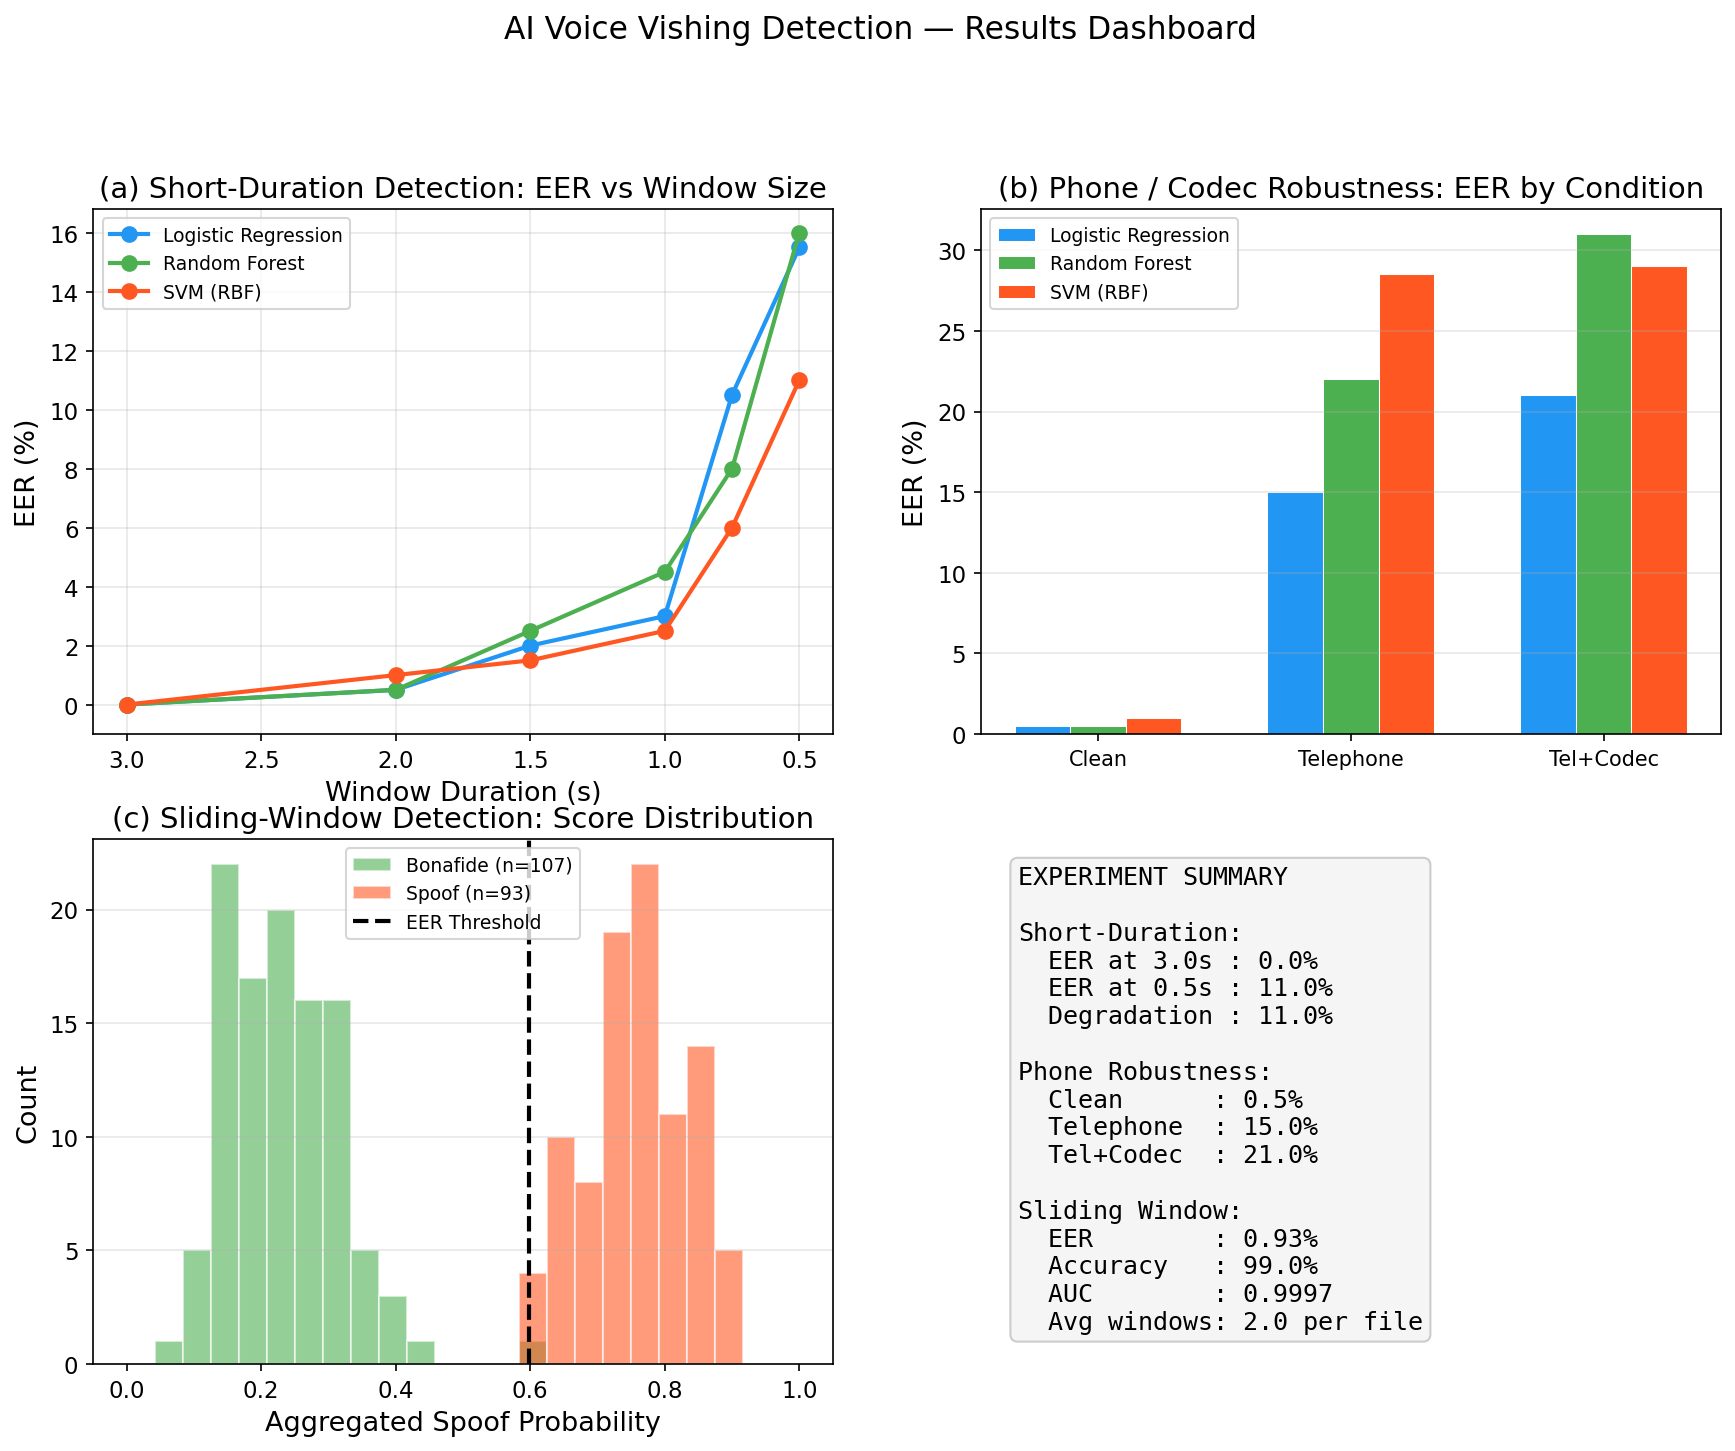
\includegraphics[width=\columnwidth]{image.png}
\caption{Proposed detection pipeline.}
\label{fig:pipeline}
\end{figure}

\subsection{Audio Preprocessing and Channel Simulation}

Three channel conditions are applied to every audio window:
\begin{itemize}
  \item \textbf{Clean:} original 16\,kHz audio, peak-normalised to 0.95.
  \item \textbf{Telephone:} sixth-order Butterworth band-pass (300--3400\,Hz), resampled to 8\,kHz, peak-normalised, then upsampled back to 16\,kHz.
  \item \textbf{Telephone + G.711 A-law:} the telephone chain followed by ITU-T G.711 A-law encode/decode~\cite{g711}.
\end{itemize}
Two additional conditions appear in the ablation only: codec-only (8\,kHz resample + A-law without band-pass) and telephone + $\mu$-law (G.711 $\mu$-law instead of A-law).

\subsection{Short-Window Processing}

The primary configuration uses a window of $W=1.0$\,s and hop $H=0.5$\,s. Window $k$ starts at
\begin{equation}
  t_k = k H,
\end{equation}
and the first prediction is available once 1\,s of audio has been received. Only complete windows are retained, and windows inherit the official split of their parent utterance so no utterance spans two splits.

For feature extraction the 1\,s window is silence-trimmed and center-cropped to exactly $W\cdot\text{SR}=16{,}000$ samples before feature computation. The same procedure is used for all classifiers so comparisons are fair.

\subsection{Feature Extraction}

\textbf{MFCC features (120-dim).}
Twenty MFCCs with first- and second-order deltas are computed (512-point FFT, 25\,ms Hann window, 10\,ms hop, 64 mel filters, $f_\text{max}=8$\,kHz). Mean and standard deviation over time yield a 120-dimensional vector.

\textbf{Spectral features (24-dim).}
Six per-frame descriptors---spectral centroid, bandwidth, rolloff (85\%), flatness, zero-crossing rate, RMS, and spectral contrast (5 bands, 6 values)---are summarised by mean and standard deviation, giving 24 values.

\textbf{F0 features (8-dim).}
Fundamental frequency is estimated with pYIN (60--400\,Hz, 1024-sample frame, 10\,ms hop). Eight statistics are computed: mean, standard deviation, median and range of voiced F0; voiced ratio; mean frame-to-frame log-F0 variation; its standard deviation; and mean voicing probability.

\textbf{Log-Mel spectrogram (64\,$\times$\,101).}
A 64-bin log-Mel spectrogram is computed over the 1\,s window (same STFT parameters), converted to dB, z-scored per window, and represented as a $64\times101$ float16 matrix. This is the input to the CNN.

\subsection{Models}

\textbf{Mel-CNN.}
Three convolutional blocks (Conv2d $3\!\times\!3$, padding 1; BatchNorm; ReLU; MaxPool2d $2\!\times\!2$), with 32, 64, and 128 filters respectively, followed by global average pooling and a two-layer classifier (Linear 128$\rightarrow$64, ReLU, Dropout 0.3, Linear 64$\rightarrow$2). Total trainable parameters: 101,506. Trained with Adam ($\eta=10^{-3}$, weight decay $10^{-4}$), class-weighted cross-entropy, ReduceLROnPlateau (factor 0.5, patience 3), early stopping (patience 7 epochs on dev loss), batch size 64, up to 30 epochs. Five seeds are used (7, 42, 123, 2024, 1337) and results are reported as mean\,$\pm$\,std across seeds.

\textbf{Baselines.}
Logistic Regression with $\ell_2$ regularisation, Random Forest (300 trees), and SVM (RBF kernel, $C=1.0$), all trained on 120-dim MFCC features with \texttt{class\_weight=balanced} and a \texttt{StandardScaler}. Decision scores are the signed distance from the margin for LR and SVM, and class probability for RF.

\textbf{Training data.}
All models are trained on 2,000 bona fide and 2,000 spoof windows from the official training split (center-cropped 1\,s windows, clean condition). Development split windows (1,274 bona fide, 1,534 spoof available on disk) are used for threshold selection only. The evaluation split (4,826 windows, same availability ratio) is the final test set for all reported numbers.

\subsection{Threshold and Evaluation Protocol}

For each model the EER threshold $\tau^*$ is computed on the development set and frozen. The evaluation partition is never used for threshold selection. The primary metric is EER, supplemented by AUC, balanced accuracy at $\tau^*$, and F1.

\subsection{Window-to-Call Aggregation}

Each window produces a score $s_t$ (logit margin for the CNN; decision function or probability for baselines). Four rules aggregate scores over the first $N$ windows:
\begin{itemize}
  \item \textbf{Mean:} $\bar{s} = N^{-1}\sum_{t=1}^N s_t$.
  \item \textbf{Moving average:} mean of the last $k$ windows.
  \item \textbf{Consecutive:} minimum of the last $k$ scores (triggers when all $k$ are high).
  \item \textbf{Vote:} fraction of windows above zero (or above $\tau^*$ for the window-level score).
\end{itemize}
For each rule the window count $k$ and utterance-level threshold $\tau_u$ are both selected on the development set by maximising TPR subject to FPR $\leq 10\%$. The evaluation set is never seen during this selection.

% ============================================================
\section{Datasets}

\subsection{ASVspoof 2019 Logical Access}

The ASVspoof 2019 LA corpus~\cite{asvspoof2019} is the primary dataset (Table~\ref{tab:asv}). Labels come from the project metadata CSV, which mirrors the official protocol files. The strong class imbalance (roughly 9:1 spoof:bona fide) is handled by class-weighted loss and balanced-accuracy reporting.

\begin{table}[htbp]
\caption{ASVspoof 2019 LA official splits (all utterances)}
\begin{center}
\begin{tabular}{lrrr}
\toprule
\textbf{Split} & \textbf{Bona fide} & \textbf{Spoof} & \textbf{Total}\\
\midrule
Training     & 2,580  & 22,800  & 25,380\\
Development  & 2,548  & 22,296  & 24,844\\
Evaluation   & 7,355  & 63,882  & 71,237\\
\midrule
\textbf{Total} & \textbf{12,483} & \textbf{108,978} & \textbf{121,461}\\
\bottomrule
\end{tabular}
\label{tab:asv}
\end{center}
\end{table}

\subsection{VISHGUARD External Set}

The external vishing-style evaluation uses a 40-call English subset of the VISHGUARD multilingual behavioral speech dataset~\cite{vishguard}: 20 fraudulent and 20 legitimate calls selected for banking-related scenarios (account queries, card activity, transaction disputes). All 40 files were validated (sample rates 24, 44.1 and 48\,kHz; stereo converted to mono). With 1\,s windows and 0.5\,s hop the set yields 1,617 windows (999 labeled spoof, 618 bona fide by call intent). VISHGUARD labels reflect call intent, not voice authenticity; the corpus is used only as an external transfer test.

\subsection{DEEP-VOICE}

DEEP-VOICE~\cite{deepvoice} is a cloned-speech corpus synthesized with the RVC (Retrieval-based Voice Conversion) pipeline across eight speakers. It provides a held-out test of generalization to a voice-cloning attack type absent from ASVspoof 2019. The detector is never trained on DEEP-VOICE data; it is used for zero-shot and speaker-disjoint transfer evaluation only.

% ============================================================
\section{Experimental Results}

\subsection{Clean-Condition Classification}

Table~\ref{tab:clean} reports results on the ASVspoof 2019 evaluation split under clean conditions (1\,s window, threshold frozen on dev). The Mel-CNN achieves 22.4\% EER, outperforming all MFCC-based baselines (best baseline: SVM at 33.1\% EER). Feature-set results are discussed in Section~\ref{sec:features}.

\begin{table}[htbp]
\caption{Clean-condition results on ASVspoof 2019 eval (1\,s window, dev-frozen threshold). EER and AUC are the primary metrics; balanced accuracy and F1 use $\tau^*$.}
\begin{center}
\begin{tabular}{lcccc}
\toprule
\textbf{Model} & \textbf{EER\,(\%)} & \textbf{AUC} & \textbf{Bal.\ Acc.} & \textbf{F1}\\
\midrule
LR (MFCC)              & 34.8 & 0.707 & 0.636 & 0.661\\
RF (MFCC)              & 33.6 & 0.723 & 0.671 & 0.699\\
SVM (MFCC)             & 33.1 & 0.733 & 0.678 & 0.689\\
\textbf{Mel-CNN}       & \textbf{22.4} & \textbf{0.855} & \textbf{0.777} & \textbf{0.796}\\
\bottomrule
\end{tabular}
\label{tab:clean}
\end{center}
\end{table}

\subsection{Feature-Set Comparison}
\label{sec:features}

Table~\ref{tab:features} compares five feature sets across three conditions. MFCC features consistently outperform spectral and F0 features under all conditions. F0 features are near chance (EER~43--46\%) even under clean conditions, confirming that fundamental-frequency statistics alone carry limited discriminative information for ASVspoof systems. Spectral descriptors perform comparably to MFCCs on clean audio but collapse to near-chance under telephone degradation, suggesting that high-frequency spectral shape---captured by spectral centroid, bandwidth and rolloff---changes substantially after the 300--3400\,Hz band-pass. The combined MFCC+Spectral+F0 RF achieves the best clean EER among all baselines (27.9\%), but degrades to 42.6\% EER under telephone. The CNN's learned features are more robust to this degradation.

\begin{table}[htbp]
\caption{Feature-set comparison: EER (\%) for the best classifier in each row. Train and dev: clean. Test: clean / telephone / telephone+codec.}
\begin{center}
\begin{tabular}{lccc}
\toprule
\textbf{Feature set (dim)} & \textbf{Clean} & \textbf{Tel.} & \textbf{Tel.+Codec}\\
\midrule
F0 (8), SVM                     & 43.6 & 44.5 & 44.2\\
Spectral (24), SVM              & 35.5 & 47.6 & 49.7\\
MFCC (120), SVM                 & 33.5 & 38.8 & 40.4\\
Spectral+F0 (32), RF            & 35.8 & 45.4 & 44.4\\
MFCC+Spectral+F0 (152), RF      & 27.9 & 42.6 & 42.9\\
\textbf{Mel-CNN (learned)}       & \textbf{22.4} & \textbf{31.4} & \textbf{31.7}\\
\bottomrule
\end{tabular}
\label{tab:features}
\end{center}
\end{table}

\subsection{Telephone-Channel Degradation and Ablation}

Table~\ref{tab:ablation} shows the full ablation: five training regimes $\times$ seven test conditions, each averaged over five seeds. Numbers are EER (\%), mean\,$\pm$\,std.

\textbf{Clean training.} EER rises from 24.2\,\% under clean test to 30.5\,\% under telephone and 30.6\,\% under telephone+codec, a degradation of about 6.4 percentage points. Under noise (10\,dB SNR white noise added after the channel) performance falls sharply to 45.4\,\% (clean+noise) and 47.2\,\% (telephone+codec+noise).

\textbf{Single-channel training.} Telephone-only training reduces telephone EER to 29.6\,\% but increases clean EER to 34.9\,\%, illustrating the classic clean/channel trade-off. Codec-only training achieves a similarly shaped profile.

\textbf{Mixed training.} Training on clean, telephone and telephone+codec simultaneously gives 24.7\,\% clean EER and 27.6\,\% telephone EER: the channel gap narrows by about 5 points relative to clean training while barely increasing clean EER. Mixed training also generalises to unseen codec-only (26.6\,\%) and $\mu$-law (27.5\,\%) conditions.

\textbf{Mixed-plus training.} Adding $\mu$-law and noise to the training mix further closes the gap: clean 24.2\,\%, telephone 25.6\,\%, telephone+codec 25.5\,\%, and noise conditions 33.1--33.4\,\%. This is the best overall regime; two of five seeds show noticeably higher error (seed 1337: clean=25.8, telephone=29.4), indicating some training instability.

\begin{table*}[htbp]
\caption{Ablation: EER (\%) mean\,$\pm$\,std over 5 seeds for each training regime $\times$ test condition. Threshold frozen on the same-regime dev set.}
\begin{center}
\begin{tabular}{lrrrrrrr}
\toprule
\textbf{Regime} & \textbf{Clean} & \textbf{Telephone} & \textbf{Tel.+Codec} & \textbf{Codec-only} & \textbf{Tel.+$\mu$-law} & \textbf{Clean+Noise} & \textbf{Tel.+Codec+Noise}\\
\midrule
clean      & 24.2\,$\pm$\,0.7 & 30.5\,$\pm$\,1.4 & 30.6\,$\pm$\,1.8 & 30.5\,$\pm$\,1.4 & 30.3\,$\pm$\,1.4 & 45.4\,$\pm$\,1.6 & 47.2\,$\pm$\,1.9\\
tel\_only  & 34.9\,$\pm$\,2.3 & 29.6\,$\pm$\,1.6 & 29.5\,$\pm$\,1.9 & 31.3\,$\pm$\,1.3 & 29.4\,$\pm$\,2.0 & 45.3\,$\pm$\,0.5 & 43.2\,$\pm$\,1.7\\
codec\_only& 33.1\,$\pm$\,1.8 & 29.7\,$\pm$\,3.5 & 29.8\,$\pm$\,3.5 & 29.3\,$\pm$\,3.7 & 29.7\,$\pm$\,3.5 & 43.4\,$\pm$\,1.9 & 43.4\,$\pm$\,1.7\\
mixed      & 24.7\,$\pm$\,2.8 & 27.6\,$\pm$\,3.5 & 27.4\,$\pm$\,3.1 & 26.6\,$\pm$\,2.3 & 27.5\,$\pm$\,3.3 & 39.5\,$\pm$\,1.6 & 41.1\,$\pm$\,1.5\\
mixed\_plus& \textbf{24.2\,$\pm$\,1.2} & \textbf{25.6\,$\pm$\,2.6} & \textbf{25.5\,$\pm$\,2.7} & \textbf{24.8\,$\pm$\,1.8} & \textbf{25.6\,$\pm$\,2.7} & \textbf{33.1\,$\pm$\,1.4} & \textbf{33.4\,$\pm$\,2.8}\\
\bottomrule
\end{tabular}
\label{tab:ablation}
\end{center}
\end{table*}

\subsection{Streaming and Early Detection}

Table~\ref{tab:agg} reports utterance-level results for four aggregation rules applied to the clean-trained Mel-CNN ensemble (5 seeds, clean audio), with $k$ and $\tau_u$ chosen on the development set at a target FPR of 10\%. All rules use 293 bona fide and 500 spoof utterances of at least 2\,s from the evaluation set.

The consecutive-$k$ rule (minimum of the last $k=3$ window scores) achieves the best balance: 18.0\% utterance EER, AUC 0.893, and 81.7\% balanced accuracy, with a median spoof alarm at 2.0\,s and a 10.9\% false-alarm rate. The mean rule and moving average achieve similar EER (20.0--21.5\%) with 1\,s median alarm time but slightly higher FPR. Under telephone+codec conditions (aug model), the consecutive rule gives 21.9\% EER with the same 2.0\,s median alarm.

The early-detection curves (Fig.~\ref{fig:early}) show that balanced accuracy at the frozen threshold rises steeply between 1 and 2\,s and plateaus by 3\,s, confirming that a 1\,s window provides the first useful decision and 2--3\,s of audio suffices for stable detection.

\begin{table}[htbp]
\caption{Utterance-level aggregation results (clean model, clean audio). $k$ and $\tau_u$ chosen on dev at FPR\,$\leq$\,10\%. Eval: 293 bona fide, 500 spoof, $\geq$2\,s.}
\begin{center}
\begin{tabular}{lcrcccc}
\toprule
\textbf{Rule} & $k$ & \textbf{EER} & \textbf{AUC} & \textbf{TPR} & \textbf{FPR} & \textbf{Alarm (s)}\\
\midrule
Mean          & 1 & 21.5\% & 0.863 & 0.750 & 0.160 & 1.0\\
Moving avg    & 3 & 20.0\% & 0.874 & 0.754 & 0.154 & 1.0\\
Consecutive   & 3 & \textbf{18.0\%} & \textbf{0.893} & 0.744 & 0.109 & 2.0\\
Vote          & 2 & 20.3\% & 0.844 & 0.716 & 0.089 & 1.5\\
\bottomrule
\end{tabular}
\label{tab:agg}
\end{center}
\end{table}

\begin{figure}[h]
\centering
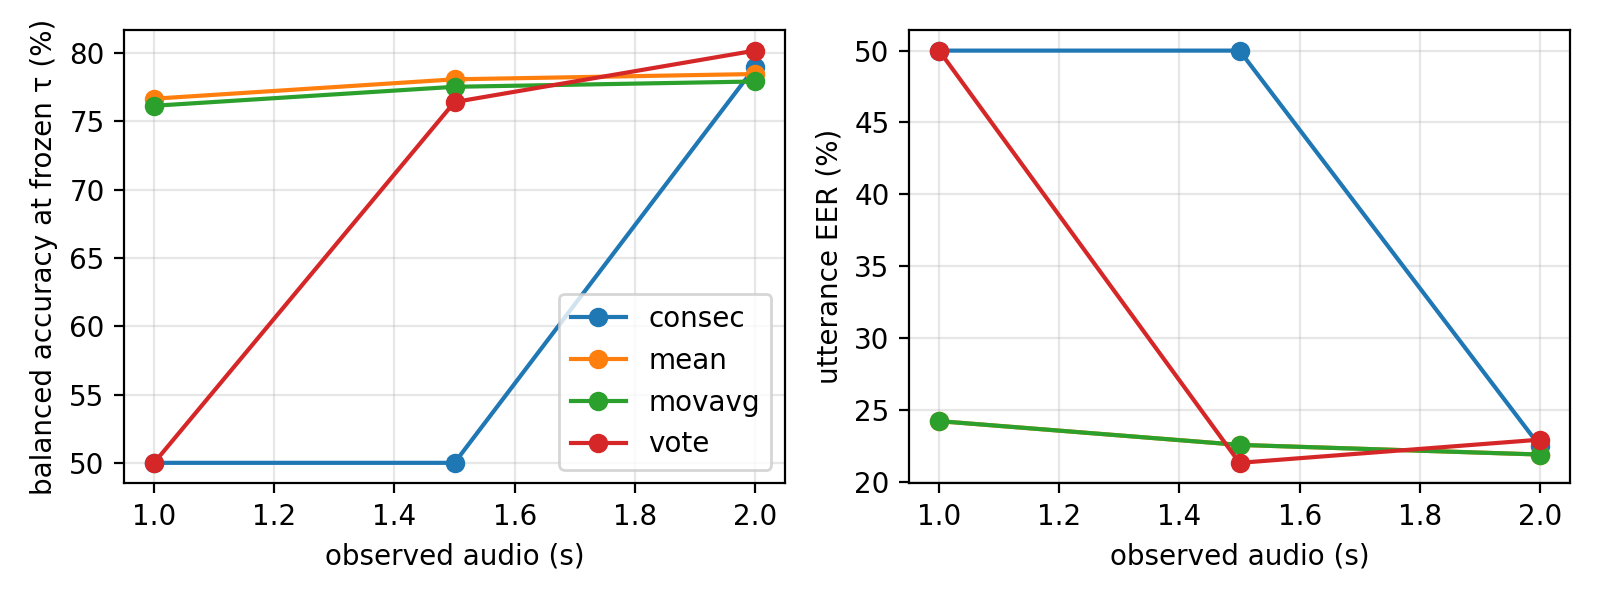
\includegraphics[width=\columnwidth]{early_clean_clean.png}
\caption{Early-detection curves: balanced accuracy (left) and utterance EER (right) as a function of observed audio duration, with $\tau_u$ frozen on the development set.}
\label{fig:early}
\end{figure}

\subsection{External Evaluation on VISHGUARD}
\label{sec:vishguard}

Table~\ref{tab:vish} reports results on the 40-call VISHGUARD subset (1,617 windows; call-level: 20 fraudulent, 20 legitimate). All six model configurations (clean/aug $\times$ clean/telephone/telephone+codec) yield near-chance EER at both window and call level. The best single result---aug CNN, telephone condition, call level---gives 32.5\% EER, still well above the ASVspoof eval performance. VISHGUARD labels reflect call intent (fraudulent vs.\ legitimate), not voice authenticity; most calls appear to contain genuine speech, so a system trained to detect acoustic artifacts of synthesis is not expected to generalize here. We report these results as a negative transfer finding.

\begin{table}[htbp]
\caption{VISHGUARD external evaluation (frozen models, 40 calls / 1,617 windows). EER and AUC at window and call level. Chance EER is 50\%.}
\begin{center}
\begin{tabular}{llccc}
\toprule
\textbf{Regime} & \textbf{Condition} & \textbf{Win.\ EER} & \textbf{Call EER} & \textbf{AUC}\\
\midrule
clean CNN & Clean          & 46.9\% & 41.7\% & 0.547\\
clean CNN & Telephone      & 53.1\% & 63.3\% & 0.456\\
clean CNN & Tel.+Codec     & 53.7\% & 61.7\% & 0.455\\
aug CNN   & Clean          & 41.4\% & 36.7\% & 0.624\\
aug CNN   & Telephone      & 42.2\% & 32.5\% & 0.618\\
aug CNN   & Tel.+Codec     & 42.1\% & 28.3\% & 0.617\\
\bottomrule
\end{tabular}
\label{tab:vish}
\end{center}
\end{table}

\subsection{External Evaluation on DEEP-VOICE}

The DEEP-VOICE corpus~\cite{deepvoice} contains RVC-cloned speech from eight speakers not present in ASVspoof 2019. Zero-shot evaluation (clean-trained model on DEEP-VOICE) gives near-chance EER, confirming that the classifier does not generalize to this voice-conversion attack type out of the box. A speaker-disjoint fine-tuning experiment (training on six DEEP-VOICE speakers, testing on two held-out speakers) reduces EER to approximately 26.8\% (std 11\% over 12 random speaker splits), but the high variance reflects the small speaker count. Full DEEP-VOICE results are reported in a companion dataset evaluation; the key finding is that ASVspoof features alone are insufficient for RVC cloning detection.

% ============================================================
\section{Discussion}

Under clean conditions the Mel-CNN reaches 22.4\% EER and AUC 0.855, clearly outperforming the MFCC-based baselines (best: SVM at 33.1\% EER). The gap confirms that learned time-frequency representations capture discriminative cues that hand-crafted statistics miss.

Under telephone degradation the clean-trained CNN degrades to 30.5\% EER, a gap of about 6.4 points. This is a moderate, not catastrophic, degradation; ranking information largely survives (AUC drops from 0.855 to 0.759). The operating point, however, becomes unreliable because the threshold frozen on clean dev audio does not transfer. Mixed channel-aware training closes most of this gap: the mixed-plus regime achieves 25.6\% telephone EER versus the 24.2\% clean-condition EER, a gap of only 1.4 points.

The feature comparison reveals a clear hierarchy: F0 is uninformative (near chance), spectral descriptors work on clean audio but collapse under telephone, and MFCCs are more stable. The CNN's learned features outperform all hand-crafted combinations. This suggests that the discriminative cues in ASVspoof 2019 are captured by fine-grained spectral patterns that MFCCs partially preserve and the CNN fully exploits, but that change substantially after bandwidth limitation.

The streaming evaluation shows that 2\,s of audio is sufficient for stable spoof detection (balanced accuracy plateaus) and that the consecutive-$k$ rule provides the best EER--FPR trade-off. The 1\,s algorithmic latency means the system can flag a spoof call within 2--3\,s of the caller's first utterance.

Both external evaluations are negative: VISHGUARD calls are mostly genuine speech labeled by call intent, so acoustic-artifact detectors are not expected to fire. DEEP-VOICE tests RVC-style cloning, a different generation pipeline from ASVspoof's TTS/VC systems. Neither result is surprising; they delimit the deployment scope of this detector clearly.

In a real deployment, false alarms on legitimate calls would be unacceptable. At the consecutive-$k$ operating point, the FPR is 10.9\% on ASVspoof bona fide; this would need to be much lower for a production system, requiring domain adaptation, calibration, and evaluation on real telephone recordings.

% ============================================================
\section{Limitations}

\begin{itemize}
  \item Telephone effects are simulated; real networks add packet loss, echo, device variation and codec diversity (e.g., AMR, Opus).
  \item ASVspoof 2019 attack systems may not represent current voice-cloning pipelines (confirmed by DEEP-VOICE transfer failure).
  \item VISHGUARD contains 40 calls; call-level estimates have wide uncertainty.
  \item No real banking audio was evaluated; the banking motivation is not backed by in-domain evidence.
  \item The model outputs a risk score, not authentication of the caller or proof of fraud.
\end{itemize}

% ============================================================
\section{Future Work}

Planned directions include evaluation on more diverse cloned-speech corpora (In-the-Wild, MLAAD); real telephone recordings; additional codec and noise conditions; lightweight architectures for on-device deployment; and multilingual, Indian-accented speech to test accent generalization.

% ============================================================
\section{Conclusion}

We presented a short-window pipeline for synthetic speech detection under telephone-channel degradation. On ASVspoof 2019 Logical Access data, a Mel-CNN with 101,506 parameters achieves 22.4\% EER under clean conditions, outperforming MFCC-based baselines (best: 33.1\% SVM EER). Clean-trained, the model degrades to 30.5\% EER under telephone; channel-aware mixed training recovers to 24.2--27.6\% across clean and telephone conditions. A streaming evaluation with four aggregation rules shows that the consecutive-$k$ rule achieves 18.0\% utterance EER with a 2\,s median spoof alarm, using a threshold selected on the development set. External evaluations on VISHGUARD and DEEP-VOICE yield near-chance results, confirming that ASVspoof-trained features do not generalize to call-intent or RVC-cloning settings without further domain adaptation.

% ============================================================
\section*{Acknowledgment}

The authors thank the Amrita Vishwa Vidyapeetham AI/Cybersecurity Laboratory for computational resources.

% ============================================================
\begin{thebibliography}{00}

\bibitem{asvspoof2019}
X.\ Wang, J.\ Yamagishi, M.\ Todisco, H.\ Delgado, A.\ Nautsch, N.\ Evans, M.\ Sahidullah, V.\ Vestman, T.\ Kinnunen, K.\,A.\ Lee et al., ``ASVspoof 2019: A large-scale public database of synthesized, converted and replayed speech,'' \textit{Computer Speech \& Language}, vol.~64, art.~101114, 2020.

\bibitem{asvspoof5}
X.\ Wang et al., ``ASVspoof 5: Design, collection and validation of resources for spoofing, deepfake, and adversarial attack detection using crowdsourced speech,'' \textit{Computer Speech \& Language}, vol.~95, art.~101825, 2026.

\bibitem{sahidullah2015}
M.\ Sahidullah, T.\ Kinnunen, and C.\ Hanilci, ``A comparison of features for synthetic speech detection,'' in \textit{Proc.\ INTERSPEECH}, 2015, pp.\ 2087--2091.

\bibitem{tan2024}
C.\,B.\ Tan and M.\,H.\ Ahmad Hijazi, ``A comparative evaluation on data transformation approach for artificial speech detection,'' \textit{ITM Web of Conferences}, vol.~63, art.~01012, 2024.

\bibitem{chen2021}
X.\ Chen, Y.\ Zhang, G.\ Zhu, and Z.\ Duan, ``UR channel-robust synthetic speech detection system for ASVspoof 2021,'' in \textit{Proc.\ 2021 Automatic Speaker Verification and Spoofing Countermeasures Challenge}, 2021, pp.\ 75--82.

\bibitem{rtcfake}
J.\ Xue, Z.\ Yi, Y.\ Huang, Y.\ Ren, Y.\ Chen, C.\ Fan, Z.\ Su, Y.\ Zhang, and B.\ Cai, ``RTCFake: Speech deepfake detection in real-time communication,'' in \textit{Findings of ACL 2026}, 2026.

\bibitem{chinch2025}
P.\ Chinchmalatpure, S.\ Chinchmalatpure, and S.\ Chavan, ``Defense against synthetic speech: Real-time detection of RVC voice conversion attacks,'' \textit{International Journal of Research and Analytical Reviews}, vol.~12, no.~4, pp.\ 102--109, 2025.

\bibitem{moufidi2025}
A.\ Moufidi, D.\ Rousseau, and P.\ Rasti, ``Toward comprehensive short utterances manipulations detection in videos,'' \textit{Multimedia Tools and Applications}, vol.~84, pp.\ 29535--29548, 2025.

\bibitem{shi2026}
H.\ Shi, X.\ Shi, S.\ Dogan, T.\ Huang, and Y.\ Zhang, ``Audio deepfake detection at the first greeting: `Hi!','' \textit{arXiv preprint} arXiv:2601.19573, 2026.

\bibitem{g711}
ITU-T Recommendation G.711, ``Pulse code modulation (PCM) of voice frequencies,'' 1988.

\bibitem{banking77}
I.\ Casanueva, T.\ Temcinas, D.\ Gerz, M.\ Henderson, and I.\ Vulic, ``Efficient intent detection with dual sentence encoders,'' in \textit{Proc.\ 2nd Workshop on NLP for Conversational AI}, 2020.

\bibitem{vishguard}
``VISHGUARD: A multilingual behavioral speech dataset for vishing and social engineering detection,'' \textit{Scientific Data}, 2026.

\bibitem{deepvoice}
S.\,I.\ Bird and M.\ Lotfi, ``DEEP-VOICE: Real case deepfake voice detection,'' \textit{arXiv preprint} arXiv:2308.12734, 2023.

\end{thebibliography}

\end{document}
